\documentclass[10pt,twocolumn]{article}

\usepackage{oxycomps}
\bibliography{references}

\pdfinfo{
    /Title (SpatialDB: A Database for Storing Dense Three-Dimensional Voxel Structures)
    /Author (Nicholas Novak)
}

\title{SpatialDB: A Database for Storing Dense Three-Dimensional Voxel Structures}
\author{Nicholas Novak}
\affiliation{Occidental College}
\email{nnovak@oxy.edu}

\begin{document}

\maketitle

\section{Introduction and Problem Context}

% What my project is
In my senior comprehensive project, I have designed and implemented a database
application that is designed specifically to store complex shapes in ``voxels'',
or three-dimensional pixels.

% Applications of voxels
A voxel\cite{enwiki:1186283262} represents a single point or cube in a
three-dimensional grid, at a variable size. This feature allows them to
approximately model many three-dimensional structures, in order to reduce the
computational complexity in analyzing the shape, which has led to many
data-related use cases outside of computer science. For example, to model the
inner workings of the brain, Neuroscientists track oxygen concentration through
neural tissue on a voxel grid as part of fMRI studies\cite{norman2006beyond},
and Movie studios such as DreamWorks use voxel data structures to model light
reflections for visual effects\cite{museth2013vdb}. The output of MRI scans in
hospitals are very high-resolution voxel grids. Most recently, machine learning
models are being trained on the LIDAR data from self-driving
cars\cite{li2020deep} in order to better process their environments. However,
voxels are not often thought of as a way to store three-dimensional shapes, and
existing research focuses mainly on efficiently representing and processing
shapes. My approach models this problem of voxel storage and representation, and
turns it into a problem of database design.

\subsection{Using Minecraft as a Model for a Database}

% The problems with Minecraft
Minecraft\footnote{https://www.minecraft.net/en-us}, released 2009, is a sandbox
game that is played in a world entirely composed of cubic voxels, where the
player has complete freedom to manipulate the world by building, destroying, or
exploring any part of it. I am focusing this database on the requirements of
Minecraft because the game involves some additional challenges that traditional
databases do not consider. Primarily, the world of Minecraft is infinite in the
horizontal $x$ and $z$ axes, but fixed in the $y$ axis, which limits the amount
of information that can be stored by the database at once. The world also
contains a denser voxel grid than in many other applications, meaning that far
more of the blocks in the world are filled than empty.

A game is also a real-time application, which means that any performance issues
will be immediately be present to the user. Most databases can be evaluated on
only their speed, but as the Minecraft server processes new information 20 times
per second, the game has a time budget of 50ms to handle all game logic,
including the storing of data. Less time processing the data in the world means
that more time will be freed up for the game to process other work, although
finishing work earlier will not necessarily be faster for the end user, if it
still under the budget of 50ms. Most databases do not meet this requirement, and
even though they may be faster, their complexity does not mean that they will
always finish operations within this time limit.

These limitations also make Minecraft unable to take advantage of a cache, since
the number of different operations that can be done on the world is infinitely
large, remembering any previous operations will often not be helpful for the
system's performance. Minecraft also provides a good benchmark for the database,
because the unpredictability of players stresses the system's ability to return
results in a variety of settings.

\section{Technical Background}

\subsection{What is a database?}
When I refer to the concept of a database, I am referencing a program that sits
more or less as a ``black box'' between the user and a software application,
storing any data required for the application. In most existing applications,
this is done by a category of databases called ``relational databases'', which
offer a very general-purpose way to store user data that is highly connected.
For instance, a person stored in a relational database would be efficiently
linked to with any of their associated information, such as name or age.

% The model of a database
In database terms, any amount of data added to the database is called a
``write'', data retrieved from the database is called a ``read'', and any
questions asked, such as ``how many people have done this'', are called
``queries''. Developers ask these questions through computer languages, one such
example being Structured Query Language or SQL, which allow
the database to be queried efficiently.

\subsection{Challenges With Existing Databases}

% Software development and SQL
Most software engineering projects start with a simple front-end and back-end,
typically implemented with some sort of Model-View-Controller architecture, and
connected to a relational SQL database \cite{sqliteOnlyDatabase}. This idea was
popularized by frameworks such as Ruby on Rails and Django, where the model was
most often modeled by structures within the database. This framework allowed
software developers to not have to worry about inner workings of the database,
and focus on writing business logic. This is how many start-ups were built, such
as GitHub \cite{githubSingleSQL}, who recently moved off its single SQL database
after 13 years, citing performance issues.

% Challenges with working with SQL: Performance
Using a single SQL-speaking database can be a significant advantage development
speed, but the database can have some issues keeping up with the demands of the
application as the performance requirements expand.
% Caching
As soon as this happens, companies typically put smaller caching applications in
front of their database, such as \verb|Redis|\footnote{https://redis.io/},
\verb|memcached|\cite{nishtala2013scaling}, or \verb|TAO| \cite{bronson2013tao},
to allow the application to remember some of the commonly asked questions and
reduce load on the database by not having to do the same work again.

\subsubsection{The Complexity of General-Purpose Databases}
% What is being done about this
Modern SQL databases are also very complex. Three of the most popular SQL
databases, PostreSQL, MySQL and Sqlite have 1.4 million lines
\footnote{https://wiki.postgresql.org/wiki/GSoC\_2018, in reference to the
text ``PostgreSQL is over 1.3M lines of code and some of the code paths can be
tricky to reach.''} of code, 2.9 million lines
\footnote{https://www.openhub.net/p/mysql}, and 150,000 lines
\footnote{https://www.sqlite.org/testing.html} respectively.

% Why are databases inefficient?
Why are databases so complex? Most of the reason for the complexity is that
because these database systems so general-purpose, they cannot assume anything
about the data stored in them. For the database, finding an efficient plan to
answer each query is a known NP-hard problem\cite{chatterji2002complexity}, and
to keep itself fast, the database must construct this plan with a complex set of
approximations, based on the assumptions that it can make, which leads to
ever-evolving complexity.

% Impossible to maintain
With this complexity, it is impossible for a single person to understand the
complete inner workings of a database. Thus, the problem of the company's
database often becomes a dedicated person in companies that can afford it, or
become entire teams of engineers at larger organizations such as
Google\cite{googlePerfTeam}.

% Intro to special-purpose databases
What happens in the larger companies that can afford more engineering time, and
have a specific problem that they cannot solve with a traditional database?
Typically, this leads to the creation of special-purpose database solutions. For
instance, the global scale of iCloud and Apple's cloud solutions required them
to create FoundationDB\cite{zhou2021foundationdb}. A different set of challenges
in the Facebook inbox led to the creation of Apache
Cassandra\cite{lakshman2010cassandra}, which is optimized to allow for many
emails to be received, at the expense of search speed, which is done far less
frequently.

\subsubsection{The Special-Purpose Database}

Limiting a database's design to a specific use-case can make the development
process much simpler, to the point where it can be done by a single person, and
can offer higher performance. The first question that needs to be asked is
whether the application is \textit{write-heavy} or \textit{read-heavy}.
Read-heavy applications occur often in web development, and most social media
platforms have far more users reading the content, than writing new content for
the platform. In contrast, write-heavy applications are often seen in analytics
workloads, where data is written from many sources, and analyzed infrequently by
users.

My application has a relatively even write and read balance, and I evaluated
three different storage data structures before choosing to implement my own

% Special-purpose databases
Recently, companies such as Tigerbeetle\cite{tigerbeetleDesign} have taken this
domain-driven approach to database design even further, while designing a
database from the ground up to do financial accounting, which outperforms a
reference MySQL implementation at 76 accounting transactions per second, to
1,757 transactions per second \cite{tigerbeetlePerf}. This highly specialized
and domain-specific approach to creating databases is what my project is going
to be based on, to create a database around the challenges that the game
Minecraft has.

\subsubsection{Key-Value Databases}

One of the main architectures that I considered for my project is a design
called a key-value store\cite{kvdatabase}, which would store the relationship of
a single voxel to its value. Many other voxel databases use this method to
achieve constant-time operations on retrieving points, which means that
regardless of the size of the dataset, the database will always be able to
return a result in the same amount of time. This structures is behind many of
the high-performance caches that are commonly used to speed up web applications,
such as Redis and RocksDB\cite{dong2021rocksdb}. In order to provide high speeds
for this data, the key-value mappings are usually stored in main memory, which
is far more expensive and limited than the system's disk drive, but offers
a speed advantage of several orders of magnitude\cite{latencyKnow}.

\section{Prior Work}

\subsection{Voxels for Efficient Computation}

Most existing literature on the topic of using voxels to store shapes focuses on
the application of the voxel grid for efficient computation. Since voxel points
are completely independent of each other, this allows for efficient parallel
processors, which are increasingly more common on consumer hardware, to take
advantage of this speedup. In VDB\cite{museth2013vdb} Museth demonstrates that
by modeling a sparse voxel grid in different resolutions, a computer cluster can
efficiently approximate a physical structures such as a cloud, in order to
calculate expensive lighting operations.

\subsection{Parallel Processing on Voxel Databases}

Williams\cite{williams1992voxel} expands upon the uses of a voxel database to
model graph and mesh-based problems. Taking advantage of the parallelism in the
grid, many problems can be reframed in the representation of voxels, and solve
those problems far more efficiently. This model however, assumes that every
voxel is stored in shared memory, making this process only viable to solve
problems that can be modeled on one machine, and are far more computationally
expensive, rather than data-intensive.

\subsection{Large Voxel Data Set Processing}

Another approach to the problem of storing voxel data is the distributed
approach in Gorte et. al. \cite{gorte2023analysis}. Since memory is limited
within one computer, this workload can be split up between many servers, which
allows very large datasets to be worked on by a single workstation through an
API. This method keeps many of the same performance considerations, but also
assumes that the voxel data is not very dense, and uses a three-dimensional
data structure called an octree, which allows the user to change the resolution
of the data that they are working on. In the paper, Gorte acknowledges the need
to split large datasets up into smaller regions, which is similar to the concept
of ``chunks'' in my implementation.

\subsection{Previous Special-Purpose Databases}

The design of my database was also inspired by the LSM tree and data-driven
designs of Tigerbeetle\cite{tigerbeetleDesign}, which is also able to handle
concurrent operations on the same design. Another database,
CockroachDB\footnote{https://www.cockroachlabs.com/product/}, uses a key-value
mapping backend to store a SQL-like tables and rows. Finally, the design of
caching layers in modern SQL caches such as Noria\cite{gjengset2018noria} show
that it it possible to efficiently remember the complex queries found in SQL,
and replicate these in real-time.

\section{Methods}

Almost every part of the database was designed so that most operations could be
done in constant time.

The database provides a simple interface to read and write data, consisting of
the following:
\begin{itemize}
  \item Read a single block
  \item Write a single block
  \item Change a range of blocks
  \item Read a pre-defined ``chunk'' of blocks
\end{itemize}


The process of fetching the data for a single point in the world starts at that
point's $x, y$ and $z$ location. The world is infinite in size on the horizontal
$x$ and $z$ axes, but limited in the vertical $y$ axis. In my database, the
world is composed of an infinite grid of ``chunks'', or columns that are a fixed
16 x 16 blocks in the $x$ and $z$ axes, but 256 blocks in the vertical $y$ axis.

Once you know a point's location, you can find with a modulus what chunk the
point is located within. From there, the database only needs to retrieve the
data for the chunk stored at that location.

Initial implementations for my database focused on tree-based approaches for
finding the files for chunks, but with their complexity and non-constant
complexity, I decided to store each chunk separately. However, with worlds with
chunk counts in the hundreds of thousands, the filesystem implementations had
issues with searching through so many files, which led to performance problems.
Finally, I settled on merging all the chunk data into one file, and use the
filesystem's \verb|seek| syscall to lookup the offset for the correct chunk. A
simple hash table was then used to store each chunk's location with its offset
in the file, which keeps the memory cost low, even with chunk counts in the
millions. This allows for constant-time searches for the chunk's data.

Once a chunk is retrieved from disk, the format of the chunk is broken down into
smaller cubic slices of the chunk, called ``sections'' each section is a
16x16x16 cubic area that keeps an index for every chunk. The point's $y$
position tells the database what section the point is in, and a simple formula
is done to convert the remaining $x$ and $z$ axes into an index within the
section.

Every section additionally stores a look-up-table, that stores a mapping of a
\textit{palette index} to the state of a block. When the value for the point is
retrieved from the section, the value returned is not the block's state, but
simply an index into this palette. The palette lookup is done in constant time,
and when a new block is added into the section that needs an additional state in
the palette, this value is added in constant time as well. The existence of this
palette supports the efficient operation of another part of the database, which
is the ability to change large portions of blocks in the world.

Once the value of the point is found in the palette, the value can be returned
to the user. A visual diagram of this process can be found in figure
\ref{fig:lookup}.

\begin{figure}
  \centering
  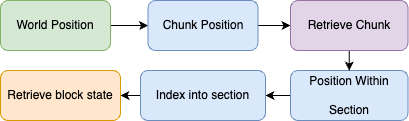
\includegraphics[width=8cm]{block-search.drawio.png}
  \caption{The process of looking up a single block}
  \label{fig:lookup}
\end{figure}

The ability to change a region of blocks is also a common operation within the
database, and which isn't locked to a specific range of chunks. This operation
is implemented as overwriting the palettes for a specific region. By overwriting
every palette index to the same value, every value in the chunk effectively gets
set to the same value. This does however create the need for an additional
``compaction'' step, where the palette is shrunk to remove duplicate values, and
every block within the section must be updated to point to the correct index in
the palette. This compaction is done upon any subsequent writes to the section
by inserting a block, because only this fixed-size section needs to be changed,
preserving the time of the operation as constant time.

Finally, the retrieval of a single chunk can be done efficiently, because the
database already stores chunks separately, and serializes these to the client.

% \cite{vohra2016apache}.

\section{Evaluation Metrics}

\subsection{Reading Single Voxels}

Reads and writes of single voxels are the most common fundamental operation for
my database, and the database should be handle this operation in the same amount
of time, regardless of the size of the world. Both my implementation and the
simpler key-value store meet this criteria.

\subsection{Changing Regions of Voxels}

Changing regions of voxels should be able to be done in linear time. This is
because resetting or changing a region of voxels is important while drawing
shapes of various resolutions. Lower resolution shapes are less precise, and
thus are able to be written faster.

\subsection{Memory Requirements}

The memory requirement is set quite low, at 256MB, in order to require the
database to store most of its data on disk, and limit its memory usage to
important caching features. This limitation was chosen for larger datasets that
don't fit within memory on a single machine, because memory is much more
expensive than disk storage, and would limit the analysis to smaller voxel grids.

\subsection{Reading Regions of Voxels}

The ability to retrieve large shapes from the database is important, because in
order to export a shape, another operation must be present to efficiently do
this. This operation therefore must be done in constant time, because as
Gorte\cite{gorte2023analysis} identifies, many researchers might want to work
on the same dataset, and exporting all this data would become inefficient for
the database to process. In the use-case of Minecraft, this allows the server to
support many more players at once, by not sending every individual block to each
client. This requirement is not met by the key-value database, but is reached by
my implementation, by sending the stored chunks on disk.

\subsection{Reading Neighboring Blocks}

The last common operation in most voxel databases is the ability to read points
that are neighboring another point. This is important because many voxel shapes
approximate cubic shapes \cite{gorte2023analysis}, and in Minecraft, players are
constantly affecting voxels that are nearer to each other.

\section{Results and Discussion}

Benchmarking on my laptop, inserting values in various spreads around the voxel
world, I get the following benchmarks, comparing an in-memory implementation of
SpatialDB, the disk-based implementation of SpatialDB, and a memory-based
key-value implementation in figure \ref{fig:reads}:

\begin{figure}
  \centering
  \begin{tabular}{c | c | c | c}
    Spread of Points & In-memory & Disk & KeyValue\\
    \hline
    128 & 4275 & 4146669 & 176.7\\
    512 & 4184 & 3319162 & 190.6\\
    2048 & 2613 & 422938 & 184.8\\
    65536 & 2382 & 18814 & 186.1
  \end{tabular}
  \caption{Time (in ns) to operate on a single voxel, based on the size of the
  world (spread)}
  \label{fig:reads}
\end{figure}

These results show that the scaling remains consistent between the in-memory
version and the key-value store, although my implementation is about two orders
of magnitude slower than the latter. This scaling is however not met by the
performance of the on-disk database. Originally, I thought that these poor
results were the result of no caching being done on the chunk files, which would
have made searches much slower, but still doesn't explain the improvement in
performance by larger worlds. This led me to implement a disk cache, which had
similar results, to the final implementation where I combined all the data in
one large file, and selectively read sections from that file. This leads me to
believe that as the points tested grow more spread out, since the world is only
so large, many points will be outside of the loaded chunks, and instantly return
empty.

This change could likely be addressed by a change in caching methods, and
remembering the data for more chunks, but this still doesn't address the slow
speeds for accessing data in the first place. The slow speeds are most likely
the decoding of the JSON data stored on disk, which is relatively large at
about 4 megabytes in size. A custom encoding method could be designed to replace
this scheme, or additionally pre-allocate the entire storage space in the
chunks, so that chunk data could be retrieved without decoding the entire chunk.
However, this would require a much more constrained data layout, and limit the
implementation of different voxels.

Additionally, compression 

\section{Ethical Considerations}

\subsection{Considerations of Computing Resources}

Since databases are at the core part of most complex systems, they are often
built to be run on hardware that the normal consumer can afford
\footnote{\url{https://docs.oracle.com/en/database/oracle/oracle-database/12.2/ntdbi/oracle-database-minimum-hardware-requirements.html}}
\footnote{\url{https://wiki.lustre.org/Lustre_Server_Requirements_Guidelines}}.

The large hardware requirements of these databases come from the environments
where they are implemented, and at many of these companies, the ability to
keep buying faster hardware allows the company to work on other things that are
more important. However, what this does to the player is effectively prices them
out of the game that they would be already playing, especially since the
database would also have to run alongside the existing Java application of
Minecraft, which quickly exhaust system memory.

In the design of my server I have to prioritize both performance to take
advantage of the existing hardware, but make sure that the accessibility for
the application does not decrease as a result.

\subsection{Considerations of Complexity}
Another factor to consider in the implementation of my database is how complex
the existing systems are. Some of the most popular SQL databases, PostgreSQL and
MySQL have 1.4 and 4.4 million lines of code respectively
\footnote{\url{https://news.ycombinator.com/item?id=24813239}}.

With so much complexity going on, this significantly decreases the overall
knowledge of the system, as well as the individual user who has to debug their
game. Most of this is from the large amount of query logic that handles caching
and speeding up certain queries, so knowing more about the specific problem that
I am trying to solve removes this process from having to be done.

Especially since most of the people in the Minecraft community are volunteers in
the open-source community, debugging this large of an application would be out of
scope for enjoying a game, and likely lead to it being replaced with something
more simple. The reliability characteristics are also less than what are
required for Minecraft, since they are being compared against a single-threaded
Java program which has been tested to do the correct thing.

\subsection{Considerations in Security}

Since these databases are very complex, there is also the risk that having a
server exposed over the internet through the Minecraft game server might leave
it exposed to attacks. While this is a large issue, an even more important
implication is the ability to configure the database correctly. Since these
databases are extremely complex, it is also very hard to make sure that they are
configured securely. There have been many high-profile data
breaches\footnote{\url{https://www.zdnet.com/article/hacker-ransoms-23k-mongodb-databases-and-threatens-to-contact-gdpr-authorities/}}
that involve a single server, even at larger companies that have dedicated teams
that involve a data breach.

My plan to mitigate this risk is to implement the database in a memory-safe
programming language, which should remove the risk class of memory-unsafety
bugs, which account for around 70\% of all bugs in the Chromium browser
engine\footnote{\url{https://www.chromium.org/Home/chromium-security/memory-safety/}},
which is entirely written in non-memory safe C++.

And if the database information is ever able to be leaked through the Minecraft
protocol, the attacker would have access to the full data, because I am planning
to store it unencrypted for performance reasons, and rely on the encryption of
the Minecraft client. And, the data involved does not involve personally
identifying information, so the usefulness of the data would be close to
nothing.

But, perhaps the most important security risk is if an attacker is able to
access the database directly and bypass all the isolation in the Minecraft
protocol, in order to wipe or corrupt the data for malicious reasons. This would
likely lead to the Minecraft server being unable to be played, and degrade the
experience of the players. It is my plan to take advantage of the limitations of
the types of Minecraft items to provide resilience and easy backups to the
system, because of the purpose-built nature of the system
\footnote{\url{https://twitter.com/eatonphil/status/1568247643788267521?s=20}}.

\subsection{Considerations in Fairness}

In the implementation of databases, it can often be beneficial to make certain
operations faster, at the expense of others that are not done as often. For
instance, if I notice that players often pull items in and out of their systems
often, but almost never search through the list of items, I can take advantage
of this to speed up the database for the most common operations. However, this
can be problematic if the things that I choose to sacrifice affect a certain
group of users.

This tradeoff between speed and reliability occurs so often in Computer Science 
and is described in terms of percentiles. For instance, if we notice that some
event occurs about half the time, we can say it is in the 50th percentile.
Similarly, if an event only occurs 1\% of the time, we can say it occurs in the
99th percentile. The impossible effect of not hurting anyone when a decision
like this is make is written about by Google \cite{dean2013tail}, who have to make every
decision like this at their scale.

My plan is to not have any tradeoffs that affect the normal gameplay of the
server, and keep it within the 50ms timeframe that the Minecraft has allocated
to itself. Apart from this, one of the main goals of the project is to give
consistent performance, so any further decisions will be made around the
existing implementation of the Minecraft server.

%https://www.embedded.com/implementing-a-new-real-time-scheduling-policy-for-linux-part-1/
%https://www.kernel.org/doc/html/latest/scheduler/sched-design-CFS.html
%https://helix979.github.io/jkoo/post/os-scheduler/

\subsection{Considerations in Accessibility}

By creating this system, I also have to consider if the players are going to
require a certain type of computer. Requiring a certain operating system or a
more powerful computer would limit access to many of the people that were
playing the game before.

However, by basing the goal of the project on improving the performance of the
already existing implementation, any improvements would result in more people
being able to play than before. Also, by designing the system for normal
hardware and in a cross-platform way, this does not limit the people that are
able to access the improvements.


\subsection{Considerations in the Concentration of Power}

With any improvements to performance to servers in Minecraft, this would allow
many of the larger hosting companies, who rent servers monthly to individual
people, to drive down their hosting costs, and allow them to have larger returns
over the smaller providers. However, since this market is so competitive between
companies, because of how easy it is to set up a company, and the options
between companies aren't very different, I would expect any improvement to be
quickly disappear into the competitive market, and benefit everyone equally.

\section{Future Work, and Conclusion}

\printbibliography

\end{document}
